\chapter{Approximation methods}
The Hamiltonian for a general neutral atom with nuclear charge $Ze$ is
\begin{equation}
\label{genham}
H=\underbrace{\sum^Z_{j=1}\lf[-\frac{\hbar^2}{2m}\onabla^2_j-\lf(\frac{1}{4\pi\epsilon_0}\frac{Ze^2}{r_j} \rt) \rt]}_{\text{kinetic energy}+\text{nuclear attraction}}+\underbrace{\vphantom{\sum^Z_{j=1}\lf[-\frac{\hbar^2}{2m}\onabla^2_j-\lf(\frac{1}{4\pi\epsilon_0}\frac{Ze^2}{r_j} \rt) \rt]}\frac{1}{2}\lf(\frac{1}{4\pi\epsilon_0} \rt)\sum_j^Z\sum^Z_{k\neq j}\frac{e^2}{|\bvec{r}_j-\bvec{r}_k|}}_{\text{interelectronic repulsion}}.
\end{equation}
The factor of $1/2$ merely corrects for the fact that the double summation counts 
over each pair twice. We then wish to solve for
\begin{equation}
H\psi(\bvec{r}_1,\bvec{r}_2,\cdots,\bvec{r}_Z)=E\psi(\bvec{r}_1,\bvec{r}_2,\cdots,\bvec{r}_Z).
\end{equation}
And the only acceptable solutions according to the symmetrisation requirement is 
when, coupled with the spin, the complete wavefunction is antisymmetric wrt 
exchange of electrons. \\
This equation cannot be solved exactly and we must resort to approximation methods 
which will be discussed in this chapter. 
\section{The variational method}
\subsection{Theory}
Consider now the ground state of an arbitrary system. The ground state \sch states
\begin{equation}
H|\psi_0\rgl=E_0|\psi_0\rgl.
\end{equation}
Right-multiplying by $\lgl\psi_0|$ we have
\begin{equation}
E_0=\frac{\lgl \psi_0|H|\psi_0\rgl}{\lgl \psi_0|\psi_0\rgl}
\end{equation}
We introduce the theorem
\begin{thrm}[The variational principle]
For \textit{any other} arbitrary function $\phi$ with the same arguments (provided 
that the integral exists of course), the corresponding energy
\begin{equation}
\label{energyphi}
E_{\phi}=\frac{\lgl \phi|H|\phi\rgl}{\lgl \phi|\phi\rgl}
\end{equation}
must have that
\begin{equation}
E_{\phi}\geq E_0,
\end{equation}
where the equality holds only for $\phi=\psi_0$.
\end{thrm}
\begin{proof}
Because the set of eigenfunctions of $H$ is complete, we can express \textit{any} 
function $\phi$ as 
\begin{equation}
|\phi\rgl=\sum^{\inf}_{n=0}  c_n|\psi_n\rgl.
\end{equation}
Where, from the orthonormality of $\psi_n$'s,
\begin{equation}
c_n=\lgl \psi_n|\phi\rgl.
\end{equation}
So \Cref{energyphi} now reads
\begin{equation}
E_{\phi}=\frac{\lgl \phi|H|\phi\rgl}{\lgl \phi|\phi\rgl}=\frac{c_n^*c_n\lgl \sum\psi_n|H|\sum \psi_n\rgl}{c_n^*c_n\lgl \sum\psi_n|\sum \psi_n\rgl}=\frac{\sum |c_n|^2E_n}{\sum |c_n|^2}.
\end{equation}
Subtracting $E_0$ from both sides, we have
\begin{equation}
E_{\phi}-E_0=\frac{\sum |c_n|^2(E_n-E_0)}{\sum |c_n|^2},
\end{equation}
which \textit{must} be non-negative as $E_n$ is by definition greater than $E_0$, 
and all $|c_n|^2$ are non-negative as well. And we obeserve that the equality 
holds necessarily when $\phi=\psi_0$ since all non-zero $c_n$'s must be $0$, but 
at $n=0$, $E_n=E_0$ also, so the entire summation in the numerator vanishes for 
all $n$. 
\end{proof}
The variational principle says that we can get an upper bound to $E_0$ by using 
any trial function as we wish, with closer approxmation if $\phi$ is functionally 
more similar to $\psi_0$. In general, we will choose a trial function that 
depends on some arbitrary \textit{variational parameters}, $\alpha,\beta,\gamma,\cdots$. The energy then will also depend upon these parameters, \ie
\begin{equation}
E_{\phi}(\alpha,\beta,\gamma,\cdots)\geq E_0.
\end{equation}
Now we can minimise $E_{\phi}$ wrt each of the parameters, so the best possible 
ground-state energy of a specific trial wavefunction can be found.
\subsection{Examples}
\textbf{Hydrogen ground state}\\
As an example, we try to approximate the hydrogen ground state wavefunction. We just need to know the Hamiltonian:
\begin{equation}
H=\frac{\hbar^2}{2m}\diff{}{r}\lf(r^2\diffp{}{r} \rt)-\frac{e^2}{4\pi\epsilon_0r}.
\end{equation}
Say we guess that the wavefunction is a Gaussian (and we know from empirical 
evidence that it will not depend on $\theta$ and $\phi$):
\begin{equation}
\phi(r)=e^{-\alpha r^2}.
\end{equation}
Let's now calculate $E_{\phi}$.
\begin{equation}
\lgl \phi|H|\phi\rgl=4\pi\intinfp\phi^*(r)H\phi(r)r^2\dif r=\frac{3\hbar^2\pi^{3/2}}{4\sqrt{2}m\alpha^{1/2}}-\frac{e^2}{4\epsilon\alpha},
\end{equation}
where we have used the standard integrals in \Cref{integrals}. Similarly, 
\begin{equation}
\lgl \phi|\phi\rgl=4\pi\intinfp\phi^*\phi r^2\dif r=\lf(\frac{\pi}{2\alpha} \rt)^{3/2}
\end{equation}
where we note that in general, these trial functions are, of course, not 
normalised, but nowhere in the derivation of the variational principal required 
that the wavefunctions, trial or actual, be normalised. \\
We can therefore compute the trial energy
\begin{equation}
E(\alpha)=\frac{3\hbar^2\alpha}{2m}-\frac{e^2\alpha^{1/2}}{\sqrt{2}\epsilon_0\pi^{3/2}}.
\end{equation}
Setting the first derivative to zero we obtain
\begin{equation}
\alpha_{\text{min}}=\frac{m^2e^4}{18\pi^3\epsilon_0^2\hbar^4},
\end{equation}
so
\begin{equation}
E_{\text{min}}=-\frac{4}{3\pi}\lf(\frac{me^4}{16\pi^2\epsilon_0^2\hbar^2} \rt)\approx-0.424\lf(\frac{me^4}{16\pi^2\epsilon_0^2\hbar^2} \rt),
\end{equation}
where the exact value is
\begin{equation}
E_0=-0.500\lf(\frac{me^4}{16\pi^2\epsilon_0^2\hbar^2} \rt).
\end{equation}
Pretty good approximation despite the wrong choice of trial function. And sure 
enough, by using the trial function of 
\begin{equation}
\phi=e^{-\alpha r}
\end{equation}
we can get the exact ground state energy and wavefunction. \\
\ \\
\textbf{Helium ground state}\\
The previous example was based on a system we do know hwo to solved exactly, and 
now we apply it to one that we don't: the helium atom, with the Hamiltonian
\begin{equation}
\begin{aligned}
H&=-\frac{\hbar^2}{2m}(\onabla^2_1+\onabla_2^2)-\frac{e^2}{2\pi\epsilon}\lf(\frac{1}{r_1}+\frac{1}{r_2} \rt)+\frac{e^2}{4\pi\epsilon_0}\frac{1}{r_{12}}\\
&=H_{1}+H_2+\frac{e^2}{4\pi\epsilon_0}\frac{1}{r_{12}},
\end{aligned}
\end{equation}
where $H_i$'s are the Hamiltonian for a single electron atom with $Z=2$, and 
they satisfy the equation
\begin{equation}
H_i\psi(r_i,\theta_i,\phi_i)=E_i\psi(r_i,\theta_i,\phi_i).
\end{equation}
We choose our trial function by ignoring the interelectronic repulsion term, \ie
\begin{equation}
\phi_0(\bvec{r}_1,\bvec{r}_2)=\psi_{1s}(\bvec{r}_1)\psi_{1s}(\bvec{r}_2),
\end{equation}
where $\psi_{1s}$ is the $Z=2$ ground state hydrogenlike wavefunction:
\begin{equation}
\psi_{1s}(\bvec{r}_i)=\lf(\frac{Z^3}{\pi a^3} \rt)^{1/2}e^{-Zr_i/a},\ i=1,2.
\end{equation}
So our trial function is 
\begin{equation}
\phi(\bvec{r}_1,\bvec{r}_2)=\frac{Z^3}{a^3\pi}e^{-Z(r_1+r_2)/a}.
\end{equation}
As the trial function is normalised this time, we only have to evaluate the 
numerator:
\begin{equation}
E(Z)=\iint \phi_0^*(\bvec{r}_1,\bvec{r}_2)H\phi_0(\bvec{r}_1,\bvec{r}_2)\dif \bvec{r}_1\dif\bvec{r}_2.
\end{equation}
This integral can seem daunting but we can greatly simplify it by realising $\psi$ 
is an eigenfunction of the hydrogenlike Hamiltonian:
\begin{equation}
H\psi=-\frac{Z^2\hbar^2}{2ma^2}\psi.
\end{equation}
We now re-write the Helium Hamiltonian in terms of hydrogenlike Hamiltonians, 
keeping in mind that $Z$ is not necessarily $2$ now as it is a variational parameter:
\begin{equation}
\begin{aligned}
H&=-\frac{\hbar^2}{2m}(\onabla^2_1+\onabla_2^2)-\frac{e^2}{2\pi\epsilon}\lf(\frac{1}{r_1}+\frac{1}{r_2} \rt)+\frac{e^2}{4\pi\epsilon_0}\frac{1}{r_{12}}\\
&=-\frac{\hbar^2}{2m}\onabla_1^2-\frac{Ze^2}{4\pi\epsilon_0r_1}-\frac{\hbar^2}{2m}\onabla_2^2-\frac{Ze^2}{4\pi\epsilon_0r_2}+\frac{(Z-2)e^2}{4\pi\epsilon_0r_1}+\frac{(Z-2)e^2}{4\pi\epsilon_0r_2}+\frac{e^2}{4\pi\epsilon_0r_{12}}\\
&=H_{Z1}+H_{Z2}+\frac{(Z-2)e^2}{4\pi\epsilon_0r_1}+\frac{(Z-2)e^2}{4\pi\epsilon_0r_2}+\frac{e^2}{4\pi\epsilon_0r_{12}}.
\end{aligned}
\end{equation}
So
\begin{equation}
\begin{aligned}
E(Z)=&\iint\phi\lf[-\frac{Z^2\hbar^2}{2ma^2}-\frac{Z^2\hbar^2}{2ma^2}+\frac{(Z-2)e^2}{4\pi\epsilon_0r_1}+\frac{(Z-2)e^2}{4\pi\epsilon_0r_2}+\frac{e^2}{4\pi\epsilon_0r_{12}} \rt]\phi\dif \bvec{r}_1\dif \bvec{r}_2\\
=&\frac{Z^6}{a^6\pi^2}16\pi^2\iint\lf[-\frac{Z^2\hbar^2}{ma^2}+\frac{(Z-2)e^2}{4\pi\epsilon_0r_1}+\frac{(Z-2)e^2}{4\pi\epsilon_0r_2} \rt]e^{-2Z(r_1+r_2)/a}r_1^2r_2^2\dif r_1\dif r_2\\
&+\frac{Z^6}{a^6\pi^2}\iint \frac{e^2}{4\pi\epsilon_0r_{12}}e^{-2Z(r_1+r_2)/a}\dif \bvec{r}_1\dif \bvec{r}_2 \\
=&\frac{16Z^6}{a^6}\iint\lf[-\frac{Z^2e^2}{4\pi\epsilon_0 a}+\frac{(Z-2)e^2}{4\pi\epsilon_0r_1}+\frac{(Z-2)e^2}{4\pi\epsilon_0r_2} \rt]e^{-2Z(r_1+r_2)/a}r_1^2r_2^2\dif r_1\dif r_2\\
&+\frac{Z^6}{a^6\pi^2}\iint \frac{e^2}{4\pi\epsilon_0r_{12}}e^{-2Z(r_1+r_2)/a}\dif \bvec{r}_1\dif \bvec{r}_2
\end{aligned}
\end{equation}
We have isolated the integral involving $r_{12}$ because they are implicitly 
dependent on $\theta$. There are four integrals to solve, for the first three we 
use the standard integral \Cref{integral1}:
\begin{equation}
\begin{aligned}
&\frac{16Z^6}{a^6}\iint-\frac{Z^2}{4\pi\epsilon_0 a}e^{-2Z(r_1+r_2)}r_1^2r_2^2\dif r_1\dif r_2\\
=&-\frac{4Z^8e^2}{\pi\epsilon_0 a^7}\lf(\int e^{-2Zr/a}r^2\dif r\rt)^2\\
=&-\frac{4Z^8e^2}{\pi\epsilon_0 a^7}\lf(\frac{a^3}{4Z^3}\rt)^2\\
=&-\frac{Z^2e^2}{4\pi\epsilon_0a}\\
=&-Z^2\lf(\frac{me^4}{16\pi^2\epsilon_0^2\hbar^2} \rt)=-Z^2\ \text{Hartree},
\end{aligned}
\end{equation}
and the second and third are the same integral:
\begin{equation}
\begin{aligned}
&\frac{16Z^6(Z-2)e^2}{4\pi\epsilon_0a^6}\iint r_1r_2^2e^{-2Z(r_1+r_2)/a}\dif r_1\dif r_2\\
=&\frac{16Z^6(Z-2)e^2}{4\pi\epsilon_0a^6}\frac{a^5}{16Z^5}\\
=&Z(Z-2)\ \text{Ha}.
\end{aligned}
\end{equation}
The last integral is trickier, we first need to choose the $z$-axis to be one of 
the vectors, say $\bvec{r}_1$, so we can use our usual spherical coordinates: 
\begin{equation}
r_{12}=(r_1^2+r_2^2-2r_1r_2\cos\theta)^{1/2}.
\end{equation}
The integral becomes
\begin{equation}
\begin{aligned}
&\frac{Z^6e^2}{4\pi^3\epsilon_0a^6}\iint\frac{1}{(r_1^2+r_2^2-2r_1r_2\cos\theta)^{1/2}}e^{-2Z(r_1+r_2)/a}\dif\bvec{r}_1\dif\bvec{r}_2\\
=&\frac{Z^6e^2}{4\pi^3\epsilon_0a^6}4\pi^2\int^{\pi}_0\sin\theta_2\dif\theta_2\intinfp\intinfp\int^{\pi}_0e^{-2Z(r_1+r_2)/a}r_1^2r_2^2\frac{\sin\theta_1\dif\theta_1\dif r_1\dif r_2}{(r_1^2+r_2^2-2r_1r_2\cos\theta_1)^{1/2}}\\
=&\frac{2Z^6e^2}{\pi\epsilon_0a^6}\intinfp\intinfp e^{-2Z(r_1+r_2)/a}r_1r_2(r_1^2+r_2^2-2r_1r_2\cos\theta_1)^{1/2}\Big|^\pi_0\dif r_1\dif r_2\\
=&\frac{2Z^6e^2}{\pi\epsilon_0a^6}\intinfp\intinfp e^{-2Z(r_1+r_2)/a}r_1r_2\lf[(r_1^2+r_2^2+2r_1r_2)^{1/2}-(r_1^2+r_2^2-2r_1r_2)^{1/2} \rt]\dif r_1\dif r_2.
\end{aligned}
\end{equation}
Now, the terms in the square brackets must be positive as we are computing 
energy. When $r_2<r_1$ we have the terms equal to $2r_2$, and when $r_2>r_1$ 
they are equal to $2r_1$. Making $r_1$ run from $0$ to infinity and splitting 
the integral over $r_2$ into two parts, the integral is 
\begin{equation}
\label{5z8}
\begin{aligned}
&\frac{2Z^6e^2}{\pi\epsilon_0a^6}\intinfp r_1e^{-2Zr_1/a}\dif r_1\lf(2\int_0^{r_1}r_2^2e^{-2Zr_2/a}\dif r_2+2r_1\int_{r_1}^{\inf}r_2e^{-2Zr_2/a}\dif r_2 \rt)\\
=&\frac{4Z^6e^2}{\pi\epsilon_0a^6}\intinfp r_1e^{-\alpha r_1}\lf[\frac{2}{\alpha^3}-\lf(\frac{r_1}{\alpha^2}+\frac{2}{\alpha^3} \rt)e^{-\alpha r_1} \rt]\dif r_1\\
=&\frac{4Z^6e^2}{\pi\epsilon_0a^6}\lf(\frac{2}{\alpha^5}-\frac{1}{4\alpha^5}-\frac{1}{2\alpha^5} \rt)\\
=&\frac{5Z}{8}\ \text{Ha}.
\end{aligned}
\end{equation}
Finally we can assemble the entire integral:
\begin{equation}
E(Z)=Z^2-\frac{27}{8}Z
\end{equation}
in Hartrees, minimising we have
\begin{equation}
Z_{\text{min}}=\frac{27}{16}\ \imp\ E_{\text{min}}\approx-2.8477.
\end{equation}
The experimental value is $-2.9033$, we have reached a pretty good approximation 
even when we have disregarded interelectronic repulsion completely. The 
variational principal in a way compensates that by returning us a $Z$ less 
than $2$, which can be understood as an \textbf{effective nuclear charge}.
\subsection{Secular determinants}
A trial function with more than one parameter can return very good results, as 
to be expected since the ground state wavefunction can be expressed as an infinite 
series of any functions, the more terms we include, the better we can approximate. 
We use a trial funciton of the form
\begin{equation}
\phi=\sum^N_{n=1}c_nf_n, 
\end{equation}
where $c_n$ are variational parameters and $f_n$ are arbitrarily chosen functions. 
We restrict ourselves to two terms, and $c_n$ and $f_n$ can be complex
\begin{equation}
\phi=c_1f_1+c_2f_2.
\end{equation}
To get $E_{\phi}$, we compute
\begin{equation}
\begin{aligned}
\lgl \phi|H\phi\rgl=&\lgl(c_1f_1+c_2f_2) |H(c_1f_1+c_2f_2) \rgl\\
=&|c_1|^2H_{11}+c_1^*c_2H_{12}+c_1c_2^*H_{21}+|c_2|^2H_{22},
\end{aligned}
\end{equation}
where 
\begin{equation}
H_{ij}=\lgl f_i|Hf_j\rgl.
\end{equation}
Similarly, 
\begin{equation}
\begin{aligned}
\lgl \phi|\phi\rgl=|c_1|^2S_{11}+c_1^*c_2S_{12}+c_1c_2^*S_{21}+|c_2|^2S_{22}.
\end{aligned}
\end{equation}
where 
\begin{equation}
S_{ij}=\lgl f_i|f_j\rgl.
\end{equation}
So we can write (to facilitate implicit differentiation)
\begin{equation}
|c_1|^2H_{11}+c_1^*c_2H_{12}+c_1c_2^*H_{21}+|c_2|^2H_{22}=E_{\phi}(|c_1|^2S_{11}+c_1^*c_2S_{12}+c_1c_2^*S_{21}+|c_2|^2S_{22}).
\end{equation}
We now minimise $E(c_1,c_2)$. However, we want the final expression to be in terms 
of $c_1$ and $c_2$, not their conjugates, purely for the sake of brevity, so 
we instead minimise $c_1^*$ and $c_2^*$:
\begin{equation}
\diffp{E}{c_1^*}=0\ \imp\ c_1(H_{11}-E{\phi}S_{11})+c_2(H_{12}-E_{\phi}S_{12})=0,
\end{equation}
and minimising $c_2^*$ we have
\begin{equation}
c_1(H_{21}-E_{\phi}S_{21})+c_2(H_{22}-E_{\phi}S_{22})=0.
\end{equation}
where we need the property, \textit{ad hoc}, that 
\begin{prt}[Complex differentiation]
\begin{equation}
\diffp fz=\frac{1}{2}\lf(\diffp fx-i\diffp fy\rt),\ \diffp{f}{z^*}=\frac{1}{2}\lf(\diffp fx+i\diffp fy\rt).
\end{equation}
\end{prt}
\begin{proof}
This is a heuristic proof and is not rigourous. See Cauchy-Riemann equation for 
theoretical foundation. Let
\begin{equation}
z\equiv x+iy,\ \imp\ z^*=x-iy, 
\end{equation}
so
\begin{equation}
x=\frac{1}{2}(z+z^*),\ y=-\frac{1}{2}i(z-z^*).
\end{equation}
So
\begin{equation}
\diffp fz=\diffp fx\diffp xz+\diffp fy\diffp yz=\frac{1}{2}\lf(\diffp fx-i\diffp fy\rt),
\end{equation}
and so on. 
\end{proof}
Anyway, casting the above equations in matrix form, we have
\begin{equation}
\begin{pmatrix}
H_{11}-E_{\phi}S_{11}&H_{12}-E_{\phi}S_{12}\\
H_{21}-E_{\phi}S_{21}&H_{22}-E_{\phi}S_{22}
\end{pmatrix}
\begin{pmatrix}
c_1\\
c_2
\end{pmatrix}=0,
\end{equation}
which means there will only be non-trivial solutions for $c_1$ and $c_2$ when 
the determinant
\begin{equation}
\begin{vmatrix}
H_{11}-E_{\phi}S_{11}&H_{12}-E_{\phi}S_{12}\\
H_{21}-E_{\phi}S_{21}&H_{22}-E_{\phi}S_{22}
\end{vmatrix}=0. 
\end{equation}
Determinants like this are called \textbf{secular determinants}. 
Expanding and solving them will give us a quadratic equation in $E_{\phi}$ without 
explicitly computing $c_n$. We take the smaller of the two solutions as the upper 
bound estimate. Once we have determined $E_{\phi}$ we can invert the matrix 
equation to find the $c_n$'s and subsequently normalise the approximate solution. 
This can be trivially generalised to trial functions of $N$ terms. \\
Just as an aside, the $f_n$'s themselves can include variational parameters to 
obtain even better approximations, but however we can't use secular determinants 
in that case and numerical computations are required. 
\subsection{The H{\" u}ckel approximations}
\label{huckel}
To compute the secular determinant more quickly, the H{\" u}ckel approximations can be used. The approximations are
\begin{enumerate}
\item The overlap integral $S_{ij}=0$ for $i\neq j$
\item The Hamiltonian matrix element is nonzero only for neighouring atoms.
\end{enumerate}
A number of simplified notations are adopted:
\begin{enumerate}
\item $H_{ii}\equiv\alpha_{ii}\equiv\alpha$
\item $H_{ij}\equiv\beta_{ij}=\beta_{ji}$
\end{enumerate}
The method proceeds as follows
\begin{enumerate}
	\item Find out the point group the molecule belongs to
	\item Identify unique sets of orbitals that are interconverted, and discard those belonging to the same symmetry species, \ie they are never interconverted
	\item Reduce the representation
	\item Set up symmetry orbitals for all sets of orbitals
	\item Solve the secular equation for symmetry orbitals belonging to the same symmetry to obtain energyies and coefficients
\end{enumerate}
This is a long list, and it best illustrated by examples
\subsubsection{Example 1}
\begin{figure}[H]
	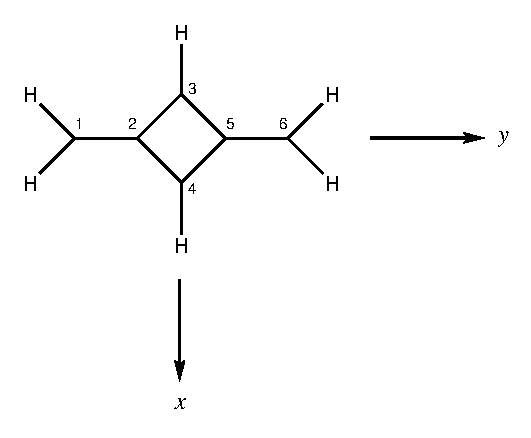
\includegraphics[width=6cm]{huckel1}
	\centering
	\caption{All the carbon atoms are sp$^2$ hybridised with the $p$ orbitals perpendicular to the plane of paper. Only $\sigma$ framework is shown on the plane of paper.}
	\label{fig:huckel1}
\end{figure}
\paragraph{Point group and basis}~\\
The molecule belongs to $D_{2h}$ point group. It is clear that the $p$-orbital pairs on atoms 1 and 6, and 2 and 5 are equivalent under operations of $D_{2h}$, so we can discard one of them since that makes reducing representations easier. The pairs 2 and 5 and 3 and 4 are not mixed or interconverted, so with them each setting up a basis, we can write
\begin{equation}
\begin{aligned}
&\Gamma_1=\phi_2+\phi_5=B_{3g}\oplus B_{1u}\\
&\Gamma_2=\phi_3+\phi_4=B_{2g}\oplus B_{1u}
\end{aligned}
\end{equation}
\paragraph{Symmetry orbitals}~\\
$B_{3g}$ transforms like $xy$, therefore the two orbitals should have opposite phase:
\begin{equation}
\begin{aligned}
&\theta_a=\tfrac{1}{\sqrt{2}}(\phi_2-\phi_5)\\
&\theta_b=\tfrac{1}{\sqrt{2}}(\phi_1-\phi_6)
\end{aligned}
\end{equation}
$B_{1u}$ transforms as $z$, so all orbitals should have the same phase:
\begin{equation}
\begin{aligned}
&\theta_c=\tfrac{1}{\sqrt{2}}(\phi_2+\phi_5)\\
&\theta_d=\tfrac{1}{\sqrt{2}}(\phi_1+\phi_6)\\
&\theta_e=\tfrac{1}{\sqrt{2}}(\phi_3+\phi_4)
\end{aligned}
\end{equation}
$B_{2g}$ transforms like $xz$, so opposite phase:
\begin{equation}
	\theta_f=\tfrac{1}{\sqrt{2}}(\phi_3-\phi_4)
\end{equation}
\paragraph{Secular equation}~\\
The secular equation for $B_{3g}$ symmetry orbitals is
\begin{equation}
	\begin{pmatrix}
		H_{aa}-E & H_{ab}\\
		H_{ba} & H_{bb}-E
	\end{pmatrix}
	\begin{pmatrix}
		c_a\\
		c_b
	\end{pmatrix}
	=0
\end{equation}
We can evaluate the matrix elements $H_{ij}$ very rapidly with the H{\" u}ckel approximations:
\begin{equation}
	H_{aa}=\alpha,\ \ H_{ab}=H_{ba}=\beta,\ \ H_{bb}=\alpha
\end{equation}
So we have
\begin{equation}
	\begin{pmatrix}
		\alpha-E & \beta\\
		\beta & \alpha-E
	\end{pmatrix}
	\begin{pmatrix}
		c_a\\
		c_b
	\end{pmatrix}
	=0
\end{equation}
Which means the secular determinant is zero. A common simplification is to divide throughout by $\beta$ and setting $(\alpha-E)/\beta=x$:
\begin{equation}
	\begin{vmatrix}
		x&1\\
		1&x
	\end{vmatrix}=0
\end{equation}
So $E=\alpha-x\beta$
\begin{equation}
	E_1=\alpha+\beta\ \ \text{or}\ \ E_2=\alpha-\beta
\end{equation}
The coefficients can be obtained easily so the overall solutions are
\begin{equation}
\begin{aligned}
	&\psi_1=\tfrac{1}{2}(\phi_1+\phi_2+\phi_5+\phi_6)\\
	&\psi_2=\tfrac{1}{2}(\phi_1-\phi_2-\phi_5+\phi_6)
\end{aligned}
\end{equation}
The $B_{1u}$ equation is
\begin{equation}
		\begin{pmatrix}
		H_{cc}-E & H_{cd} &H_{ce}\\
		H_{dc} & H_{dd}-E &H_{de}\\
		H_{ec} & H_{ed} & H_{ee}-E
	\end{pmatrix}
	\begin{pmatrix}
		c_c\\
		c_d\\
		c_e
	\end{pmatrix}
	=0
\end{equation}
The diagonal matrix elements $H_{ii}$ always come to $\alpha$, the off-diagonal terms are
\begin{equation}
	H_{cd}=\beta\ \ H_{ce}=2\beta\ \ H_{de}=0
\end{equation}
So the simplified secular equation is
\begin{equation}
		\begin{pmatrix}
		x & 1 &2\\
		1 & x &0\\
		2 & 0 & x
	\end{pmatrix}
	\begin{pmatrix}
		c_c\\
		c_d\\
		c_e
	\end{pmatrix}
	=0
\end{equation}
$E=\alpha-x\beta$ so $E=\alpha$, $E=\alpha\pm\sqrt{5}\beta$. The coefficents can be solved but is too laborious to get into.\par
The $B_{2g}$ secular matrix is 1 by 1, so the energy is just $E=\alpha$. We can draw up the energy level diagram as
\begin{figure}[H]
	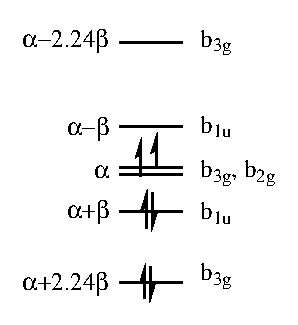
\includegraphics[width=6cm]{huckel2}
	\centering
	\caption{There are a total of 6 $p_{\pi}$ electrons in the system, with atoms 3 and 4 formally radicals.}
	\label{fig:huckel2}
\end{figure}
And we define the \emph{delocalisation energy} as
\begin{defi}[Delocalisation energy]
The delocalisation energy is the difference between the energy of the fully delocalised system and the putative system where only localised double bonds exist.
\end{defi}
So for this system, as we have seen, a localised double bond MO between the same element have two levels, $E=\alpha+\beta$ and $E=\alpha-\beta$, so a two-electron bond have $2\beta+2\beta$. In the localised version of this system, there are two two-electron double bonds and two radical atoms, which just have energies of $\alpha$, so the delocalisation energy is
\begin{equation}
	E_{\text{delocalisation}}=E_{\text{delocalised}}-E_{\text{localised}}=6\alpha+2(\sqrt{5}+1)\beta-(6\alpha+4\beta)\approx2.47\beta
\end{equation}
\section{Perturbation theory}
\subsection{Nondegenerate theory}
Say we are unable to solve
\begin{equation}
H\psi=E\psi,
\end{equation}
however we do have exact solutions for
\begin{equation}
H^{(0)}\psi_n^{(0)}=E_n^{(0)}\psi_n^{(0)}, 
\end{equation}
where $H^{(0)}$ should be broadly functionally similar to $H$. 
We omit the subscript $n$ for now for simplicity's sake. 
This means we can write the original Hamiltonian as $H^{(0)}$ and the difference:
\begin{equation}
H=H^{(0)}+\lambda H',
\end{equation}
where the first term is called the \textbf{unperturbed Hamiltonian} and the 
difference is called the \textbf{perturbation}. $\lambda$ is simply a 
dimensionless parameter running from $0$ to $1$, and it should be small for the 
perturbed system to resemble the unperturbed system. We therefore hope to solve
\begin{equation}
(H^{(0)}+\lambda H')\psi=E\psi.
\end{equation}
If $\lambda$ is small, we can write 
\begin{subequations}
\begin{align}
\psi&=\psi^{(0)}+\lambda\psi^{(1)}+\lambda^2\psi^{(2)}+\cdots\\
E&=E^{(0)}+\lambda E^{(1)}+\lambda^2E^{(2)}+\cdots, 
\end{align}
\end{subequations}
where, formally (added for clarity, rarely used)
\begin{subequations}
\begin{align}
E^{(k)}&=\frac{1}{k!}\diff[k]{E^{(0)}}{\lambda}\Big|_{\lambda=0}\\
\psi^{(k)}&=\frac{1}{k!}\diff[k]{\psi^{(0)}}{\lambda}\Big|_{\lambda=0}.
\end{align}
\end{subequations}
So, the \sch has now become
\begin{equation}
\begin{aligned}
(H^{(0)}+\lambda H')&(\psi^{(0)}+\lambda\psi^{(1)}+\lambda^2\psi^{(2)}+\cdots)\\
=(E^{(0)}+\lambda E^{(1)}+\lambda^2E^{(2)}+\cdots)&(\psi^{(0)}+\lambda\psi^{(1)}+\lambda^2\psi^{(2)}+\cdots).
\end{aligned}
\end{equation}
Expanding and collecting like terms of $\lambda$ we have 
\begin{subequations}
\begin{align}
&H^{(0)}\psi^{(0)}=E^{(0)}\psi^{(0)}\ (\lambda^0\ \text{terms})\\
&H^{(0)}\psi^{(1)}+H'\psi^{(0)}=E^{(0)}\psi^{(1)}+E^{(1)}\psi^{(0)}\ (\lambda^1\ \text{terms})\label{1stpert}\\
&\cdots\nonumber
\end{align}
\end{subequations}
\Cref{1stpert} reads, in bra-ket notation
\begin{equation}
\label{h0h1}
H^{(0)}|\psi^{(1)}\rgl+H'|\psi^{(0)}\rgl=E^{(0)}|\psi^{(1)}\rgl+E^{(1)}|\psi^{(0)}\rgl.
\end{equation}
Multiplying with the bra $\lgl\psi^{(0)}$ we have
\begin{equation}
\begin{aligned}
\lgl\psi^{(0)} |H^{(0)}\psi^{(1)}\rgl+\lgl\psi^{(0)} |H'\psi^{(0)}\rgl&=E^{(0)}\lgl\psi^{(0)} |\psi^{(1)}\rgl+E^{(1)}\lgl\psi^{(0)} |\psi^{(0)}\rgl\\
\lgl H^{(0)}\psi^{(0)} |\psi^{(1)}\rgl+\lgl\psi^{(0)} |H'\psi^{(0)}\rgl&=E^{(0)}\lgl\psi^{(0)} |\psi^{(1)}\rgl+E^{(1)}\\
E^{(1)}&=\lgl\psi^{(0)} |H'\psi^{(0)}\rgl, 
\end{aligned}
\end{equation}
where in the second line we have use the hermiticity of the Hamiltonian. 
We now have the theorem
\begin{thrm}[First-order perturbation theory]
\label{1stpert}
For known perturbed operator $H'$ and known unperturbed eigenfunction 
$\psi^{(0)}$, the first-order correction in energy, $E^{(1)}$ is given by
\begin{equation}
E^{(1)}=\lgl \psi^{(0)}|H'\psi^{(0)}\rgl.
\end{equation}
\end{thrm}
We now have the energy correction, what about the correction in wavefunction? We rewrite \Cref{h0h1} as 
\begin{equation}
\label{1stpertrew}
(H^{(0)}-E^{(0)}_n)\psi^{(1)}_n=-(H'-E^{(1)}_n)\psi_n^{(0)}, 
\end{equation}
where we have added the $n$ subscript where it did not really matter before. 
This is essentially an inhomoheneous differential equation for $\psi_n^{(1)}$. 
We try expanding $\psi_n^{(1)}$ in $\psi_n^{(0)}$'s as we know they form a 
complete set: 
\begin{equation}
\psi^{(1)}_n=\sum_{m\neq n}c_m^{(n)}\psi^{(0)}_m.
\end{equation}
We need to exclude the $m=n$, \ie $\psi^{(0)}_n$ term because the normalisation 
requirement for $\psi_n$ requires that
\begin{equation}
1=\lgl \psi_n|\psi_n\rgl=\lgl \psi^{(0)}_n |\psi^{(0)}_n\rgl+\lambda(\lgl\psi^{(1)}_n|\psi^{(0)}_n\rgl+\lgl \psi^{(0)}_n|\psi^{(1)}_n\rgl)+\lambda^2(\cdots)+\cdots,
\end{equation}
but since the first term of the sum must be $1$ due to orthonormality of the 
unperturbed state, the subsequent terms must be zero, which means 
\begin{equation}
\label{pertorth}
\lgl \psi^{(1)}_n|\psi^{(0)}_n\rgl=0, 
\end{equation}
which means $\psi^{(1)}_n$ cannot contain a $\psi^{(0)}_n$ term. Now putting this 
into \Cref{1stpertrew} we get
\begin{equation}
\begin{aligned}
\sum_{m\neq n}(E_m^{(0)}-E_n^{(0)})c_m^{(n)}\psi_m^{(0)}&=-(H'-E_n^{(1)})\psi_n^{(0)}\\
\sum_{m\neq n}(E_m^{(0)}-E_n^{(0)})c_m^{(n)}\lgl\psi_l^{(0)}|\psi_m^{(0)}\rgl&=-\lgl\psi_l^{(0)}|H'\psi_n^{(0)}\rgl+E_n^{(1)}\lgl\psi_l^{(0)}|\psi_n^{(0)}\rgl
\end{aligned}
\end{equation}
If we set $l=n$ we recover the energy correction since the left side will return 
zero. But if $l\neq n$, we get
\begin{equation}
(E_l^{(0)}-E_n^{(0)})c_l^{(n)}=-\lgl\psi_l^{(0)} |H'\psi_n^{(0)} \rgl, 
\end{equation}
which gives us expression for the $c_m^{(n)}$'s (by relabelling) and so we have what we're looking for: 
\begin{thrm}[First-order correction in wavefunction]
\begin{equation}
\psi_n^{(1)}=\sum_{m\neq n}\frac{\lgl\psi_m^{(0)} |H'\psi_n^{(0)} \rgl}{(E_n^{(0)}-E_m^{(0)})}\psi_m^{(0)}.
\end{equation}
\end{thrm}
Going one power higher we have
\begin{equation}
\begin{aligned}
H^{(0)}\psi_n^{(2)}+H'\psi_n^{(1)}&=E_n^{(0)}\psi_n^{(2)}+E_n^{(1)}\psi_n^{(1)}+E_n^{(2)}\psi_n^{(0)}\\
\lgl\psi_n^{(0)}|H^{(0)}\psi_n^{(2)}\rgl+\lgl\psi_n^{(0)}|H'\psi_n^{(1)}\rgl&=E_n^{(0)}\lgl\psi_n^{(0)}|\psi_n^{(2)}\rgl+E_n^{(1)}\lgl\psi_n^{(0)}|\psi_n^{(1)}\rgl+E_n^{(2)}\lgl\psi_n^{(0)}|\psi_n^{(0)}\rgl\\
E_n^{(0)}\lgl\psi_n^{(0)}|\psi_n^{(2)}\rgl+\lgl\psi_n^{(0)}|H'\psi_n^{(1)}\rgl&=E_n^{(0)}\lgl\psi_n^{(0)}|\psi_n^{(2)}\rgl+E_n^{(1)}\lgl\psi_n^{(0)}|\psi_n^{(1)}\rgl+E_n^{(2)}\\
E_n^{(2)}&=\lgl\psi_n^{(0)}|H'\psi_n^{(1)}\rgl-E_n^{(1)}\lgl\psi_n^{(0)}|\psi_n^{(1)}\rgl
\end{aligned}
\end{equation}
but as we have already seen in \Cref{pertorth}, the second term shall be zero, so
\begin{equation}
\begin{aligned}
E_n^{(2)}&=\sum_{m\neq n}c_m^{(n)}\lgl \psi_n^{(0)} |H'\psi_m^{(0)} \rgl \\
&=\sum_{m\neq n}\frac{\lgl\psi_m^{(0)} |H'\psi_n^{(0)} \rgl\lgl\psi_n^{(0)} |H'\psi_m^{(0)} \rgl}{E_n^{(0)}-E_m^{(0)}}\\
&=\sum_{m\neq n}\frac{|\lgl\psi_m^{(0)} |H'\psi_n^{(0)} \rgl|^2}{E_n^{(0)}-E_m^{(0)}}
\end{aligned}
\end{equation}
\begin{thrm}[Second-order energy correction]
\label{2ndecorr}
\begin{equation}
E_n^{(2)}=\sum_{m\neq n}\frac{|\lgl\psi_m^{(0)} |H'\psi_n^{(0)} \rgl|^2}{E_n^{(0)}-E_m^{(0)}}.
\end{equation}
\end{thrm}
Now, all of this will crumble if $E_n^{(0)}=E_m^{(0)}$, \ie if there are two 
\textbf{degenerate} unperturbed states. We will discuss it after we look at some 
examples. 
\subsection{Examples}
\textbf{Anharmonic oscillators}\\
The Hamiltonian is now given by 
\begin{equation}
H=\underbrace{-\frac{\hbar^2}{2\mu}\diff[2]{}{x}+\frac{1}{2}kx^2}_{H^{(0)}}\underbrace{\vphantom{-\frac{\hbar^2}{2\mu}\diff[2]{}{x}+\frac{1}{2}kx^2}+\frac{1}{6}\gamma x^3+\frac{1}{24}bx^4}_{H'}.
\end{equation}
And we know that the unperturbed ground wavefunction is
\begin{equation}
\psi^{(0)}(x)=\lf(\frac{\alpha}{\pi}\rt)^{1/4}e^{-\alpha x^2/2}
\end{equation}
where $\alpha=(k\mu/\hbar^2)^{1/2}$. \\
So we apply the first order perturbation theory:
\begin{equation}
\begin{aligned}
E^{(1)}=&\lgl \psi^{(0)}|H'\psi^{(0)} \rgl\\
=&\lf(\frac{\alpha}{\pi}\rt)^{1/2}\bigg[\frac{\gamma}{6}\underbrace{\intinf x^3e^{-\alpha x^2}\dx}_{\text{odd integrand, }0}+\frac{b}{24}\intinf x^4e^{-\alpha x^2}\dx \bigg]\\
=&\frac{b}{32\alpha^2}=\frac{\hbar^2b}{32k\mu}, 
\end{aligned}
\end{equation}
where we have used the standard integral. So the first order ground-state energy is 
\begin{equation}
E=\frac{1}{2}\hbar\omega+\frac{1}{32}\frac{\hbar^2b}{k\mu}.
\end{equation}
\ \\
\textbf{Helium ground state (again)}\\
The unperturbed Hamiltonian is 
\begin{equation}
H^{(0)}=H_1+H_2
\end{equation}
where the $H_i$'s are $Z=2$ hydrogenlike Hamiltonians, and the unperturbed ground state and energy are
\begin{equation}
\begin{aligned}
\psi^{(0)}=\psi_{1s}(r_1,\theta_1,\phi_1)\psi_{1s}(r_2,\theta_2,\phi_2)\\
E^{(0)}=-\frac{Z^2}{2}-\frac{Z^2}{2},
\end{aligned}
\end{equation}
and the perturbed Hamiltonian is 
\begin{equation}
H'=\frac{e^2}{4\pi\ep r_{12}}.
\end{equation}
Applying the theory we have
\begin{equation}
E^{(1)}=\iint\psi_{1s}(\bvec{r}_1)\psi_{1s}(\bvec{r}_2)\frac{e^2}{4\pi\ep r_{12}}\psi_{1s}(\bvec{r}_1)\psi_{1s}(\bvec{r}_2)\dif\bvec{r}_1\dif\bvec{r}_2=\frac{5}{8}Z,
\end{equation}
where we have used the same result from \Cref{5z8}. So the first-order energy is 
\begin{equation}
E=-Z^2+\frac{5}{8}Z=-2.75.
\end{equation}
Slightly worse than the variational calculation we did earlier, but with higher 
order corrections the energy will become highly accurate. 
\subsection{Degenerate theory}
This section draws heavily from L2.3-3.2 of \cite{bartonyt} in conjunction with 
its accompanying notes (\cite{barton}) and also Section 6.8 of \cite{atkinsqm}.\par
Now suppose we have an $N$-fold degeneracy of the \textit{unperturbed} 
wavefunction, which is to say, for $1<k<N$
\begin{equation}
H^{(0)}|n^{(0)},k\rgl=E^{(0)}|0,k\rgl, 
\end{equation}
this is the same as saying that $H^{(0)}$ is, in the basis of the eigenstate, 
a diagonal matrix with digonal entries
\begin{equation}
H^{(0)}=\text{diag}\{E_1^{(0)},E_2^{(0)},\cdots,\underbrace{E_n^{(0)},\cdots,E_n^{(0)}}_{N},\cdots \}.
\end{equation}
In the \textit{degenerate subspace}, $\mathbb{V}_N$, we choose a collection of 
$N$ \textit{orthonormal} eigenstates
\begin{equation}
|n^{(0)};1\rgl,|n^{(0)};2\rgl,\cdots,|n^{(0)};N\rgl.
\end{equation}
The other states outside the subspace may also contain degeneracy but we do not 
have to be concerned with them, since they have \textit{different energy} than 
\textit{these} degenerate states, and so do not pose problems in the denominator, 
so to say. We label this space $\hat{V}$, with eigenvectors (and since $H^{(0)}$ 
is diagonal in $\hat{V}$, the basis vectors) $|p^{(0)}\rgl $. 
Compactly put, the total state space (Hilbert space) is
\begin{equation}
\mathcal{H}=\mathbb{V}_N\oplus\hat{V}.
\end{equation}
We will use the following orthonormality conditions: 
\begin{prt}[Orthonormality conditions of DPT]
\label{dptorth}
\begin{equation}
\lgl p^{(0)} |q^{(0)} \rgl=\delta_{pq},\ \lgl p^{(0)} |n^{(0)};k \rgl=0,\ \lgl n^{(0)};k |n^{(p>0)};k \rgl=0,
\end{equation}
\end{prt}
where the third is due to \Cref{pertorth} again, which intuitively says that the 
higher order terms receive no correction from the ground state, because it can 
just be reabsorbed into the normalisation of the ground state (just a restatement 
of the justification of \Cref{pertorth}). 
However note that it can receive correction from \textit{other} degenerate states, 
\ie $\lgl n^{(0)};k |n^{(p>0)};k \rgl$ is not necessarily zero.\par
In the most general terms, when the perturbation ($\lambda$) is turned on, 
the degenerate states and their energies will become
\begin{equation}
\begin{aligned}
|n^{(0)};k\rgl\rightarrow|n;k\rgl_{\lambda}&\equiv|n^{(0);k}+\lambda|n^{(1)};k\rgl+\lambda^2|n^{(2)};k\rgl+O(\lambda^3)\\
E_n^{(0)}\rightarrow E_{n,k}(\lambda)&\equiv E_n^{(0)}+\lambda E_{n,k}^{(1)}+\lambda^2 E_{n,k}^{(2)}+O(\lambda^3)
\end{aligned}
\end{equation}
Now, we say that the degeneracy is \textit{lifted} in the first order if all 
$E_{n,k}^{(1)}$ has different values, \ie they have now diverged and can be told apart. 
Our goal is find these corrections and then the first-order corrections in the 
eigenvector, $|n^{(1)};k\rgl $, for all $k$. \par
To cast this in the eigenfunction language we've used for the nondegenerate case, this is 
to say that we will determine the linear combinations of $\psi^{(0)}_k$'s that make up 
$\psi^{(1)}_k$, and implicitly in this we also need to find an 
\textit{appropriate set} of $\psi^{(0)}_k$'s such that our final linear 
combinations will be as simple as possible.\par
The \sch to solve is
\begin{equation}
H(\lambda)|n;k\rgl_{\lambda}=E_{n,k}(\lambda)|n;k\rgl_{\lambda},
\end{equation}
where
\begin{equation}
H(\lambda)=H^{(0)}+\lambda H',
\end{equation}
is just our Hamiltonian with perturbation as before. We'll extract our equations 
in ascending orders of $\lambda$ exactly as before: 
\begin{subequations}
\begin{align}
&\lambda^0:(H^{(0)}-E_n^{(0)})|n^{(0)};k\rgl=0,\\
&\lambda^1:(H^{(0)}-E_n^{(0)})|n^{(1)};k\rgl=(E_{n,k}^{(1)}-H')|n^{(0)};k\rgl ,\\
&\lambda^2:(H^{(0)}-E_n^{(0)})|n^{(2)};k\rgl=(E_{n,k}^{(1)}-H')|n^{(1)};k\rgl+E_{n,k}^{(2)}|n^{(0)};k\rgl,\\
&\cdots\nonumber
\end{align}
\end{subequations}
The $\lambda^0$ equation is trivial, and we can ignore it. Now we have a 
three-step plan to solve our problem at hand:
\begin{enumerate}
	\item Right-multiply the $\lambda^1$ equation with $\lgl n^{(0)};l|$, conclude condition that the choice of basis must fulfill.
	\item Use the $\lambda^1$ equation to get the components of $|n^{(1)};k\rgl$ in $\hat{V}$.
	\item Right-multiply the $\lambda^2$ equation with $\lgl n^{(0)};l|$ to get the second order energy correction $E^{(2)}_{n,k} $ and the component of $\lgl n^{(0)};l|$ in $\mathbb{V}_N$.
\end{enumerate}
\textbf{Step 1}\\
The LHS is simply zero due to the orthonormality condition and the hermiticity of $H^{(0)}$. \par
The RHS yields
\begin{equation}
\label{6240}
\lgl n^{(0)};l|(E^{(1)})_{n,k}-H'|n^{(0)};k \rgl=0\ \imp\ 
(H')_{lk}=E_{n,k}^{(1)}\delta_{lk}
\end{equation}
Now this equation tells us several very important things, the most important being
\begin{thrm}[Diagonalisation of $H'$]
$H'$ is diagonalised in $\mathbb{V}_N$, and the first order correction in energy is 
\begin{equation}
E_n^{(1)}=(H')_{nk,nk}, 
\end{equation}
the diagonal entries of $H'$ \textit{in the choice of basis} in 
$\mathbb{V}_N$ that diagonalises $H'$. The $n$ subscript is just to 
remind us that there's an $n$-fold degeneracy. 
\end{thrm}
There are three additional remarks:
\begin{enumerate}
	\item We have only shown that $H'$ is diagonalised in $\mathbb{V}_N$ \textit{only}, it is \textbf{not} diagonalised on the entire Hilbert space $\mathcal{H}$, \ie the basis vectors $|n^{(0)};k$ are eigenvectors only in $\mathbb{V}_N$ not $\mathcal{H}$. We can see this by inserting a resolution of identity:
	\begin{equation}
	\begin{aligned}
	H'|n^{(0)};l\rgl\Big|_{\mathcal{H}}&=\sum_q |n^{(0)};q\rgl \lgl n^{(0)};q |H'|n^{(0)};l \rgl\Big|_{\mathbb{V}_N}+\sum_p |p^{(0)}\rgl \lgl p^{(0)}|H' |n^{(0)};l \rgl\Big|_{\hat{V}}\\
	&=\sum_q E_{n,l}^{(1)}\delta_{lq}|n^{(0)};q\rgl+\sum_p |p^{(0)}\rgl \lgl p^{(0)}|H' |n^{(0)};l \rgl\\
	&=E_{n,l}^{(1)}|n^{(0)};l\rgl+\sum_p |p^{(0)}\rgl \lgl p^{(0)}|H' |n^{(0)};l \rgl
	\end{aligned}
	\end{equation}
	If we only resolved the identity in $\mathbb{V}_N$ we will have gotten the first term only, which means that it's diagonalised in it. The second term means that $|n^{(0)};k\rgl$ indeed have components along $\hat{V}$, \ie it receives contribution from other states, which intuitively makes sense. 
	\item As we can see, we can \textit{only} determine the energy correction if $H'$ is diagonalised. This requires the choice of a `good' basis set of $|n^{(0)};k\rgl$'s, as alluded to before. If we fail to choose a good basis set we just have to manually diagonalise it. 
	\item This relates to the above point, we can utilise a theorem, introduced below to determine if $H'$ is diagonal without much computation. If it's not, however, we'll have to manually diagonalise it, which will be discussed below. 
\end{enumerate}
\begin{thrm}[Quick determination of whether $H'$ diagonalises]
The matrix $H'$ is diagonal for a choice of basis in $\mathbb{V}_N$ if there is a 
Hermitian operator $K$ that commutes with $H'$ for which the chosen basis vectors are 
eigenstates of $K$ with \textit{different} eigenvalues. 
\end{thrm}
\begin{proof}
Let $[H',K]=0$ and that for two basis states in $\mathbb{V}_N$, $|n^{(0)};p\rgl$ and $|n^{(0)};q\rgl$ we have eigenvalues of $K$, $\lambda_p\neq\lambda_q$, so we have
\begin{equation}
0=\lgl n^{(0)};p|[H',K]|n^{(0)};q \rgl=\underbrace{(\lambda_p-\lambda_q)}_{\neq0}\lgl n^{(0)};p|H'|n^{(0)};q \rgl.
\end{equation}
Therefore the off-diagonal entries of $H'$ must vanish. 
\end{proof}
Now, if we weren't so lucky to choose an orthonormal basis, all we need to do is to examine the elements of $H'$ in $\mathbb{V}_N$ and calculate the roots of the 
\textit{characteristic equation}, which we can then use to diagonalise the matrix. \par
\textbf{Step 2}\\
We now determine the components of $|n^{(1)};k\rgl$ along $\hat{V}$, whose basis vectors 
are $\rgl p^{(0)}|$, so we right-multiply it to the equation to find
\begin{equation}
\begin{aligned}
\lgl p^{(0)} | (H^{(0)}-E_n^{(0)})|n^{(1)};k \rgl\Big|_{\hat{V}}&=-\lgl p^{(0)} | H'|n^{(0)};k \rgl\\
(E_p^{(0)}-E_n^{(0)})\lgl p^{(0)} | n^{(1)};k \rgl\Big|_{\hat{V}}&=-(H')_{p,nk}\\
|n^{(1)};k\rgl\Big|_{\hat{V}}&=-\sum_p\frac{(H')_{p,nk}}{E_p^{(0)}-E_n^{(0)}}|p^{(0)}\rgl\\
|n^{(1)};k\rgl=|n^{(1)};k\rgl\Big|_{\mathbb{V}_N}+|n^{(1)};k\rgl\Big|_{\hat{V}}&=-\sum_p\frac{(H')_{p,nk}}{E_p^{(0)}-E_n^{(0)}}|p^{(0)}\rgl+|n^{(1)};k\rgl\Big|_{\mathbb{V}_N}
\end{aligned}
\end{equation}
\textbf{Step 3}\\
Now we want to find the components in the degenerate space, so we right-multiply the 
$\lambda^3$ equation with the basis vectors $\lgl n^{(0)};l|$:
\begin{equation}
\begin{aligned}
0=&\lgl n^{(0)};l | (E^{(1)}_{nk}-H')|n^{(1)};k \rgl+E^{(2)}_{nk}\delta_{kl}\\
=&-\lgl n^{(0)};l | (E^{(1)}_{nk}-H')\sum_p|p^{(0)} \rgl\frac{(H')_{p,nk}}{E_p^{(0)}-E_n^{(0)}}\\
&+\lgl n^{(0)};l | (E^{(1)}_{nk}-H')|n^{(1)};k \rgl\Big|_{\mathbb{V}_N}+E^{(2)}_{nk}\delta_{kl}\\
=&\lgl n^{(0)};l | H'\sum_p|p^{(0)} \rgl\frac{(H')_{p,nk}}{E_p^{(0)}-E_n^{(0)}}+\lgl n^{(0)};l | (E^{(1)}_{nk}-H')|n^{(1)};k \rgl\Big|_{\mathbb{V}_N}+E^{(2)}_{nk}\delta_{kl}\\
=&\sum_p\frac{(H')_{nl,p}(H')_{p,nk}}{E_p^{(0)}-E_n^{(0)}}+\lgl n^{(0)};l | (E^{(1)}_{nk}-H')|n^{(1)};k \rgl\Big|_{\mathbb{V}_N}+E^{(2)}_{nk}\delta_{kl}.
\end{aligned}
\end{equation}
To simply this expression further we insert a resolution of identity in the second term
\begin{equation}
\begin{aligned}
&\lgl n^{(0)};l | H'|n^{(1)};k \rgl\Big|_{\mathbb{V}_N}\\
=&\underbrace{\lgl n^{(0)};l | H'|\bigg(\sum_q|n^{(0)};q \rgl}_{(H')_{nl,nq}} \lgl n^{(0)};q+\sum_p|p^{(0)}\rgl\underbrace{\vphantom{\bigg(\sum_q}\lgl p^{(0)}| \bigg)|n^{(1)};k\rgl\Big|_{\mathbb{V}_N}}_{\hat{V}\perp\mathbb{V}_N\ \imp\ 0}\\
=&\sum_q E^{(1)}_{nl}\delta_{lq}\lgl n^{(0)};q | n^{(1)};k \rgl\Big|_{\mathbb{V}_N}.
\end{aligned}
\end{equation}
So we obtain the `master' equation:
\begin{equation}
\underbrace{-\sum_p\frac{(H')_{nl,p}(H')_{p,nk}}{E_p^{(0)}-E_n^{(0)}}+(E_{nk}^{(1)}-E_{nl}^{(1)})}_{\text{known quantities}}\underbrace{\vphantom{-\sum_p\frac{(H')_{nl,p}(H')_{p,nk}}{E_p^{(0)}-E_n^{(0)}}}\lgl n^{(0)};l | n^{(1)};k \rgl\Big|_{\mathbb{V}_N}}_{\text{main unknown}}+E_{nk}^{(2)}\delta_{lk}=0.
\end{equation}
This equation is quite rich in information: we can obtain the second-order energy 
correction if we set $l=k$, which elimintates our main unknown due to the third 
orthonormality condition. When we set $l\neq	k$ the second-order energy disappears, 
leaving us a simpler expression for our main unknown.
\begin{thrm}[Second-order energy correction, degenerate]
When $l=k$, we immediately obtain
\begin{equation}
\begin{aligned}
E^{(2)}_{nk}&=\lgl n^{(0)};k | H'|n^{(1)};k \rgl\Big|_{\hat{V}}\\
&=-\sum_p\frac{|(H')_{nk,p}|^2}{E_p^{(0)}-E_n^{(0)}},
\end{aligned}
\end{equation}
We see that it's the same form as the nondegenerate case (\Cref{2ndecorr}), 
only that the sum is over outside the degenerate space. 
\end{thrm}
As an aside, if we believed naively that there are no components inside the degenerate 
space, we would have concluded that
\begin{equation}
\lgl n^{(0)};l | H'|n^{(1)};k \rgl\Big|_{\hat{V}}=0, 
\end{equation}
which we have shown to be not zero. \par
Finally, we set $l\neq k$ to get
\begin{equation}
\begin{aligned}
\lgl n^{(0)};l | n^{(1)};k \rgl\Big|_{\mathbb{V}_N}&=\frac{1}{E_{nk}^{(1)}-E_{nl}^{(1)}}\lgl n^{(0)};l | H'|n^{(1)};k \rgl\Big|_{\hat{V}}\\
&=-\frac{1}{E_{nk}^{(1)}-E_{nl}^{(1)}}\sum_p\frac{(H')_{nl,p}(H')_{p,nk}}{E_p^{(0)}-E_n^{(0)}},\ l\neq k
\end{aligned}
\end{equation}
The fraction implies that the degeneracy must be \textit{completely} lifted, otherwise 
we must resolve the degeneracy to higher orders. Projecting along the basis we have
\begin{equation}
|n^{(1)};k\rgl\Big|_{\mathbb{V}_N}=-\sum_{l\neq k}|n^{(0)};k\rgl\frac{1}{E_{nk}^{(1)}-E_{nl}^{(1)}}\sum_p\frac{(H')_{nl,p}(H')_{p,nk}}{E_p^{(0)}-E_n^{(0)}}.
\end{equation}
Curiously the degenerate corrections depend on the nondegenerate corrections. In all, 
\begin{thrm}[First-order correction to eigenfunction, degenerate]
\begin{equation}
\begin{aligned}
|n^{(1)},k\rgl&=|n^{(1)},k\rgl\Big|_{\mathbb{V}_N}+|n^{(1)},k\rgl\Big|_{\hat{V}}\\
&=-\sum_{l\neq k}|n^{(0)};k\rgl\frac{1}{E_{nk}^{(1)}-E_{nl}^{(1)}}\sum_p\frac{(H')_{nl,p}(H')_{p,nk}}{E_p^{(0)}-E_n^{(0)}}-\sum_p\frac{(H')_{p,nk}}{E_p^{(0)}-E_n^{(0)}}|p^{(0)}\rgl
\end{aligned}
\end{equation}
\end{thrm}
\section{The Hartree-Fock method}
\subsection{Self-consistent field method}
\label{scf}
A more inspired trial function for the variational method could be the 
\textbf{Slater orbitals}, given by 
\begin{equation}
S_{nlm}(r,\theta,\phi)=Nr^{n-1}e^{-\zeta r}Y^m_l(\theta,\phi),
\end{equation}
where $\zeta$ is a variational parameter and
\begin{equation}
N=\frac{(2\zeta)^{n+1/2}}{\sqrt{(2n)!}}.
\end{equation}
There is no inclusion of the Legendre polynomial so there are't any radial nodes, 
and as a consequence these orbitals aren't in general orthogonal. \\
Now the starting point of the Hartree-Fock procedure for helium is to write the 
two-electron wavefunction as a product of two orbitals, typically linear 
combinations of slater orbitals:
\begin{equation}
\psi(\bvec{r}_1,\bvec{r}_2)=\phi(\bvec{r}_1)\phi(\bvec{r}_2).
\end{equation}
The two one-electron wavefunctions are the same, which is \textit{in direct violation} of the Pauli exclusion principle. We ignore it for the moment. 
We must try to account for the interelectronic repulsion in the Hamiltonian:
\begin{equation}
\label{hfham}
H_1=-\frac{1}{2}\onabla_1^2-\frac{2}{r}+V_1^{\text{eff}}(r_1),
\end{equation}
where we have adopted atomic units and where the effective potential is where we 
introduce interelectronic repulsion as an average potential (this is also known as 
the \textit{mean field approximation}):
\begin{equation}
V^{\text{eff}}_1(r_1)=\lgl \phi(\bvec{r}_2)|\frac{1}{r_{12}}|\phi(\bvec{r}_2)\rgl.
\end{equation}
Now we have our \sch
\begin{equation}
H_1\phi(\bvec{r}_1)=\epsilon_1\phi(\bvec{r}_1).
\end{equation}
This is called the \textbf{Hartree-Fock equation} for a Helium atom. A special 
feature of the equation is that its Hamiltonian depends on $\phi(\bvec{r}_2)$ 
through \Cref{hfham}. $\phi(\bvec{r}_2)$ in turn is the exact same function as the 
solution of the equation, $\phi(\bvec{r}_1)$. This recursive relation allows for 
iteration and that's the essence of the \textbf{self-consistent field method}: we 
first guess a form, any form, for $\phi(\bvec{r}_2)$ and evaluate the effective 
potential, and hence the Hamiltonian, and we solve the \sch for $\phi(\bvec{r}_1)$
, by \hl{todo/todo-supo: check if by variational principle or perturbation theory}, and use the output as the 
input again, until the output is sufficiently close to the input, or \textit{
self-consistent}. 
\subsection{Accounting for spin}
\label{acc_for_spin}
In treating the helium atom just now we only used the spatial part of the trial 
wavefunction, and it appeared to have contradicted Pauli exclusion principle. 
But we have not, we just need to say that the two electrons must be in the 
singlet configuration, which is antisymmetric wrt electron exchange. The spin 
does not contribute anything to any integrals involving spatial integration 
as the Hamiltonian does not depend on it\footnote{This is again assuming spin and 
orbitals are uncoupled.} and that they are made orthonormal. \\
However, all this triplet and singlet talk is when we only have two electrons, 
what if we need to construct antisymmetric wavefunctions out of $N$-electrons? 
We introduce the 
\begin{defi}[Slater determinant]
We can use the Slater determinant to construct antisymmetric $N$-electron wavefunctions:
\begin{equation}
\ups(1,2,\cdots,N)=\frac{1}{\sqrt{N!}}
\begin{vmatrix}
u_1(1)&u_2(1)&\cdots&u_N(1)\\
u_1(2)&u_2(2)&\cdots&u_N(2)\\
\vdots&\vdots&\ddots&\vdots\\
u_1(N)&u_2(N)&\cdots&u_N(N)
\end{vmatrix}, 
\end{equation}
where $u_i(j)$ are the $i$-th complete (\ie spin included) orthonormal orbitals 
for particle $j$. 
\end{defi} 
The determinant works because
\begin{enumerate}
	\item It changes signs whenever two electrons (rows) are swapped; 
	\item It vanishes whenever two electrons occupy the same state (two identical columns). 
\end{enumerate}
For example, we look at the lithium atom. The intuition tells us to try 
\begin{equation}
\psi(\bvec{r}_1,\bvec{r}_2,\bvec{r}_3)=\phi_{1s}(\bvec{r}_1)\phi_{1s}(\bvec{r}_2)\phi_{1s}(\bvec{r}_3), 
\end{equation}
but we the Pauli exclusion principle says we can't possibly accomodate three 
electrons in the $1s$ orbital, and we put our electron in the next lowest energy 
orbital\footnote{This is still just to construct a trial wavefunction because we don't know for sure what the energy level is like for lithium atoms, but it's the best guess we've got.}, the $2s$, and construct the antisymmetric wavefunction as follows:
\begin{equation}
\psi=\frac{1}{\sqrt{3!}}
\begin{vmatrix}
1s\alpha(1)&1s\beta(1)&2s\alpha(1)\\
1s\alpha(2)&1s\beta(2)&2s\alpha(2)\\
1s\alpha(3)&1s\beta(3)&2s\alpha(3)
\end{vmatrix}, 
\end{equation}
where $1s$ is shorthand for $\psi_{1s}$ and $\alpha$ is shorthand for spin-up and $\beta$ for spin-down. \\
Now let's treat the first excited state of helium, $1s^12s^1$. \\
First we introduce a more compact notation\cite{hughbanks}:
\begin{equation}
1s\equiv1s\alpha,\ \overline{1s}\equiv1s\beta
\end{equation}
and
\begin{equation}
|1s\ \overline{2s}|\equiv N
\begin{vmatrix}
1s(1)&\overline{2s}(1)\\
1s(2)&\overline{2s}(2)\\
\end{vmatrix}, 
\end{equation}
where the normalisation constant is implied. 
Now let's construct the antisymmetric wavefunctions: 
\begin{equation}
|1s\ 2s|=\frac{1}{\sqrt{2}}
\begin{vmatrix}
1s\alpha(1)&2s\alpha(1)\\
1s\alpha(2)&2s\alpha(2)
\end{vmatrix}\propto[1s(1)2s(2)-2s(1)1s(2)](\uparrow\uparrow)\ (^3\ups,\ M_s=+1)
\end{equation}
\begin{equation}
|1s\ \overline{2s}|=\frac{1}{\sqrt{2}}
\begin{vmatrix}
1s\alpha(1)&2s\beta(1)\\
1s\alpha(2)&2s\beta(2)
\end{vmatrix}\propto1s(1)2s(2)\uparrow\downarrow-2s(1)1s(2)\downarrow\uparrow
\end{equation}
Now this is a state with $M_s=0$ according to \Cref{add_zmom}, if we combine a particle 
with spin up and one with spin down we get zero $z$-momentum. And here's one more
\begin{equation}
|\overline{1s}\ 2s|\propto1s(1)2s(2)\downarrow\uparrow-2s(1)1s(2)\uparrow\downarrow.
\end{equation}
Now, this is the \textbf{decoupled picture}, in which $m$, the $z$-spin momenta 
are specified, which is a perfectly legitimate way to specify the system, but we 
would like to speak of `singlet' and `triplet', \ie of the \textbf{coupled 
picture} where $s$, the total spin momentum is specified, to do so we take the 
linear combination of our states:
\begin{equation}
\begin{aligned}
&\frac{1}{\sqrt{2}}(|1s\ \overline{2s}|+|\overline{1s}\ 2s|)=[1s(1)2s(2)-2s(1)1s(2)](\uparrow\downarrow+\downarrow\uparrow)\ (^3\ups,\ M_s=0) \\
&\frac{1}{\sqrt{2}}(|1s\ \overline{2s}|-|\overline{1s}\ 2s|)=[1s(1)2s(2)-2s(1)1s(2)](\uparrow\downarrow-\downarrow\uparrow)\ (^1\ups,\ M_s=0)
\end{aligned}
\end{equation}
The last state is
\begin{equation}
|\overline{1s}\ \overline{2s}|\propto[1s(1)2s(2)-2s(1)1s(2)]\downarrow\downarrow\ (^3\ups, M_s=-1).
\end{equation}
Ok, let's apply first-order perturbation theory to these orbitals. \hl{todo: read atkinsqm on degenerate cases, dk if this is entirely correct, priority: high}:
\begin{equation}
\begin{aligned}
E^{(1)}=&\lgl \ups_{\pm}|\frac{1}{r_{12}}|\ups_{\pm}\rgl\\
=&\frac{1}{2}\lgl1s(1)2s(2)\pm2s(1)1s(2)|\frac{1}{r_{12}}|1s(1)2s(2)\pm2s(1)1s(2)\rgl\\
\equiv&J\pm K, 
\end{aligned}
\end{equation}
where $J$ is the \textbf{Coulomb integral} and $K$ the \textbf{exchange integral} 
(Section 7.9 of \cite{atkinsqm}):
\begin{equation}
\begin{aligned}
J&=\lgl 1s(1)2s(2)|\frac{1}{r_{12}}|1s(1)2s(2)\rgl\\
K&=\lgl 1s(1)2s(2)|\frac{1}{r_{12}}|1s(2)2s(1)\rgl
\end{aligned}
\end{equation}

\subsection{The Hartree-Fock method}
In \Cref{scf} we have discussed the Hartree-Fock method for the helium atom. 
However it is only a special case as the spin and spatial wavefunction neatly 
separates:
\begin{equation}
\ups=\frac{1}{\sqrt{2}}
\begin{vmatrix}
1s\alpha(1)&1s\beta(1)\\
1s\alpha(2)&1s\beta(2)
\end{vmatrix}
=\frac{1}{\sqrt{2}}1s(1)1s(2)(\uparrow\downarrow-\downarrow\uparrow).
\end{equation}
And it is readily seen that the same is impossible for even lithium atom as the the dependences of all the spatial wavefunctions will be permuted. \hl{todo-supo: can we introduce LCs like above?}\\
Now we are ready to introduce the general Hartree-Fock method. Our goal is still the same: to solve the \sch with Hamiltonian (same as in \Cref{genham}):
\begin{equation}
H=\sum_i H^{(0)}(i)+\frac{1}{2}\sum_{i\neq j}\frac{1}{r_{ij}}, 
\end{equation}
where the first term is the \textit{core Hamiltonian} with nuclear charge $Ze$ for 
the $i$-th electron, and the second term is the interelectronic repulsion. 
By using the slater determinant to approximate the orbitals and by using the 
mean-field approximations for effective interelectronic potentials, and through 
some tricky derivation (see pp. 528-531 of \cite{atkinsqm}) the completely general 
Hartree-Fock equation is introduced as follows:
\begin{thrm}[Hartree-Fock equation]
The Hartree-Fock equation for a \textit{spin-orbital}\footnote{The spins will 
produce Kronecker deltas anyway, but it's just more correct to speak of 
spin-orbitals.} $\phi_s(1)$ occupied by electron 1 is 
\begin{equation}
\lf[H^{(0)}(1)+\sum_r(J_r-K_r) \rt]\phi_s(1)=\epsilon_s\phi_s(1),
\end{equation}
where the sum is over all occupied spin-orbitals. 
\end{thrm}
$J$ and $K$ are two operators, defined as follows:
\begin{defi}[Coulomb and exchanger operators]
\ \\
$J_r$ is the \textbf{Coulomb operator}
\begin{equation}
J_r|\phi_s(1)\rgl=\lgl\phi_r(2)|\frac{1}{r_{12}}|\phi_r(2)\rgl|\phi_s(1)\rgl.
\end{equation}
$K_r$ is the \textbf{exchange operator}
\begin{equation}
K_r|\phi_s(1)\rgl=\lgl\phi_r(2)|\frac{1}{r_{12}}|\phi_s(2)\rgl|\phi_r(1)\rgl.
\end{equation}
$J$ accounts for the effect of Coulombic repulsion and $K$, spin correlation. 
\end{defi}
Note that since 
\begin{equation}
J_a(1)|\phi_a(1)\rgl=K_a(1)|\phi_a(1), 
\end{equation}
the sum in the Fock operator correctly gives results for all electron pair interactions without counting the same electron interacting with itself. \\
Now the Fock operator depends on $n$ spin-orbitals, and again we solve the 
Hartree-Fock equation by the self-consistent field method. After that, the 
Fock operator is theoretically a well-defined Hermitian operator and we can 
generate an infinite set of eigenfunctions, but in practice we only solve 
$m\geq n$ optimised spin-orbitals, with the $n$ lowest energy orbitals called 
\textbf{occupied orbitals} and the rest \textbf{virtual orbitals}. The slater 
determinant (or a linear combination of them, to correct the spin symmetry) 
composed with the optimised $n$ occupied orbitals is then the 
HF ground-state wavefunction for the system, $\Phi_0$. \\
The HF-SCF method takes into account spin correlation, however, the Coulombic 
interactions between electrons are treated in an average way, so no instantaneous 
interactions, nor quantum mechanical electron distribution, are taken into 
account. These are collectively called \textbf{electron correlation}, and is 
entirely left out of the picture by the HF-SCF method. 